\documentclass{article}
\usepackage[legalpaper, portrait, margin=1in]{geometry}
\usepackage{graphicx}
\title{CSCI 2270 Final Project}
\author{Nicholas Wroblewski}
\date{13 December 2020}
\setlength{\parskip}{2em}

\newlength\tindent
\setlength{\tindent}{\parindent}
\setlength{\parindent}{0pt}
\renewcommand{\indent}{\hspace*{\tindent}}

\begin{document}
\begin{titlepage}
\maketitle
\thispagestyle{empty}
\end{titlepage}

\newpage
\setcounter{page}{1}
\section*{Introduction}
    \begin{abstract}
        
        \noindent In this final project, different data structures will be implemented to keep track of integer-based patient ID's. The focus is to measure which structure is the most applicable for the given use case. The performance will be measured by analyzing the timings for each structure's functions. In part A, databases will be implemented, and in part B, sort algorithms will be implemented. 
    \end{abstract}
    
    \textbf{Part A:}
        Two databases will be constructed: a hash table and a doubly linked list. Search and insert times will be analyzed to distinguish which method is the most efficient. 
        
     \textbf{Part B:}
    Two sort algorithms will be implemented: bubble sort and heap sort. Sort and insert times will be analyzed to see which method is the most efficient. 
    
\newpage

\section*{Part A: The Hash Table and Doubly Linked List}
Below are the timing figures for the hash table and the doubly linked list. Lastly, the search and insert times are compared for each method. 

\begin{figure}[!htb]
    \centering
    \includegraphics{DLL}
    \caption{Insert and search times for the doubly linked list. Note the different time scales.}
\end{figure}

\hfill \break

\begin{figure}[!htb]
    \centering
    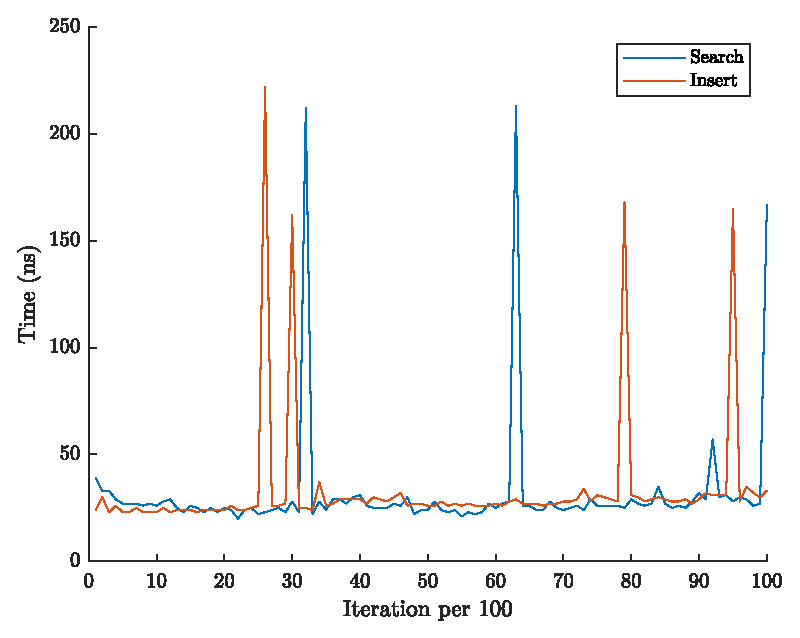
\includegraphics{hashBoth.eps}
    \caption{Insert and search times for the hash table.}
\end{figure}

\hfill \break

\newpage

\begin{figure}[!htb]
    \centering
    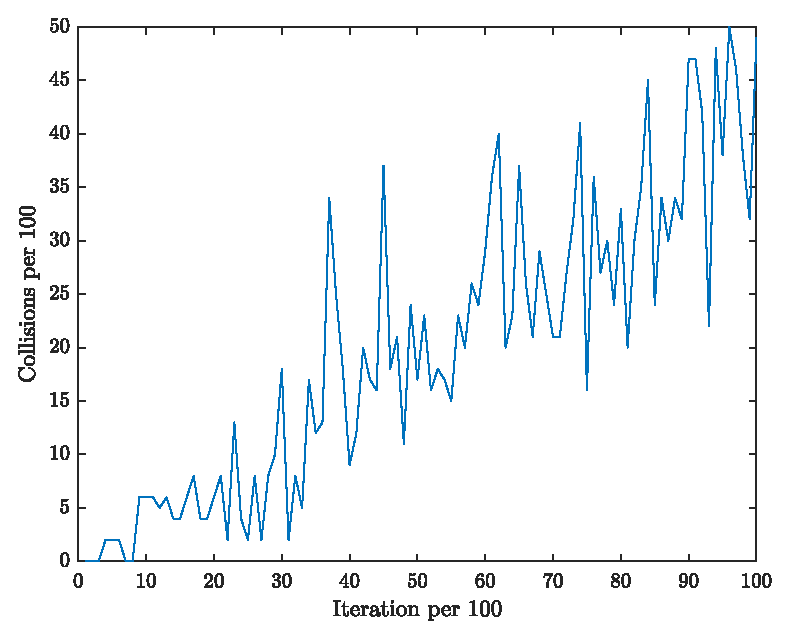
\includegraphics[height=30em]{HashCollisions.eps}
    \caption{Quadratic collisions for the hash table while inserting.}
\end{figure}


As expected, the number of collisions increases as the number of entries increases. Taking the integral of this graph would provide the total number of collisions after inserting all of the data. 

\newpage

\begin{figure}[!htb]
    \centering
    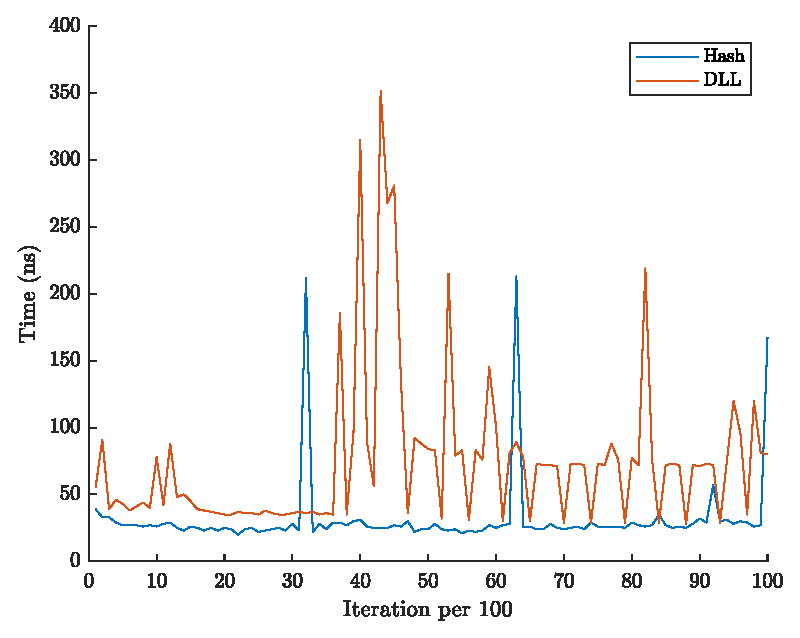
\includegraphics[height=30em]{HashDLLInsert.eps}
    \caption{Insert timings for the doubly linked list and hash table.}
\end{figure}


As seen, both insert times are comparable. The doubly linked list inserts the new node at the head of the list, so inserting is quick, with complexity \( O(1) \). The doubly linked list's increased insert time is most likely due to the fact that memory must be allocated when inserting a new node. Multiple collisions while inserting an element in the hash table causes the spikes in insert times. On average, hash table insertions have complexity \( O(1) \), and \( O(n) \) in its worst case. 
\hfill \break

\begin{figure}[!htb]
    \centering
    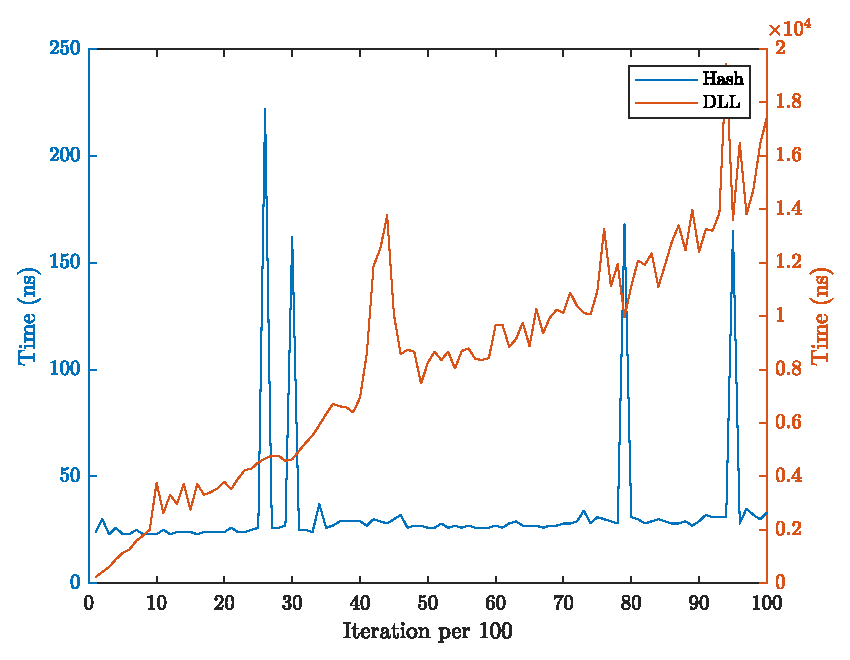
\includegraphics[height=30em]{HashDLLSearch.eps}
    \caption{Search timings for the doubly linked list and hash table. Note the different time scales.}
\end{figure}

As for search times, the hash table exceeds the doubly linked list. This is because the doubly linked list must look at every node and check if the key matches the searched value, giving it complexity \( O(n) \). The hash table's array implementation allows the data to be accessed in constant time when no probing occurs. On average, search times are \( O(1) \), and \( O(n) \) in the worst case. Delayed search times for the hash table occur when there are multiple collisions while probing. 

\newpage

\section*{Part B: Bubble Sort and Heap Sort}
Below are the timing figures for the bubble sort and heap sort. Lastly, the sort and insert times are compared for each method. 

\begin{figure}[!htb]
    \centering
    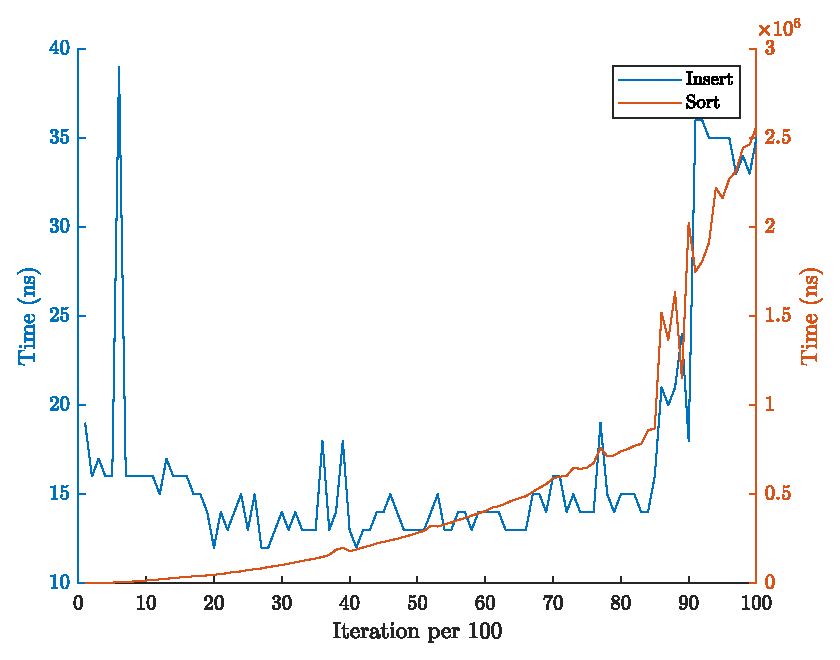
\includegraphics[height=30em]{Bubble.eps}
    \caption{Sort and Insert timings for bubble sort. Note the different time scales.}
\end{figure}

\hfill \break

\begin{figure}[!htb]
    \centering
    \includegraphics[height=30em]{Heap.eps}
    \caption{Sort and Insert timings for heap sort. Note the different time scales.}
\end{figure}

\newpage

\begin{figure}[!htb]
    \centering
    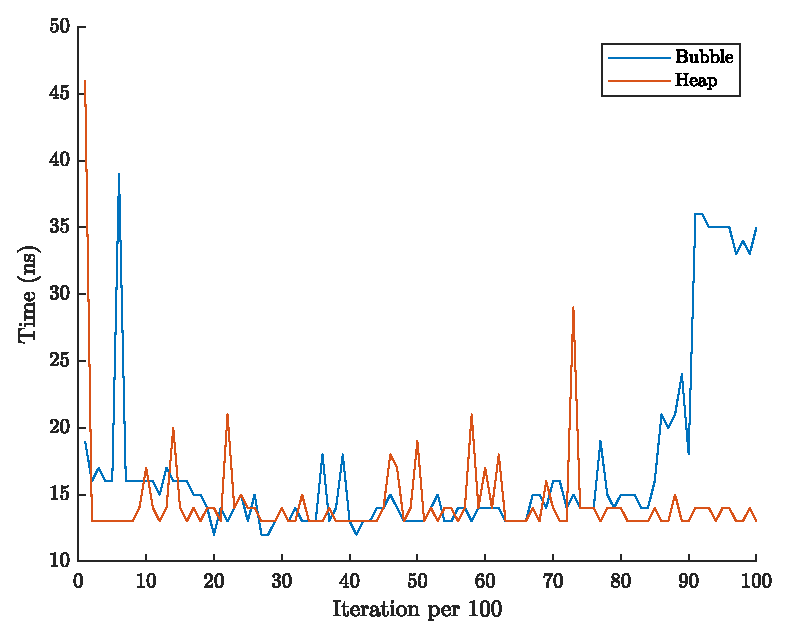
\includegraphics[height=30em]{BubbleHeapInsert.eps}
    \caption{Insert timings for heap sort and bubble sort.}
\end{figure}

As shown, insert times are quick for both methods. Since both methods insert the new data at the end of the array, both insert times have complexity \( O(1) \).

\hfill \break

\begin{figure}[!htb]
    \centering
    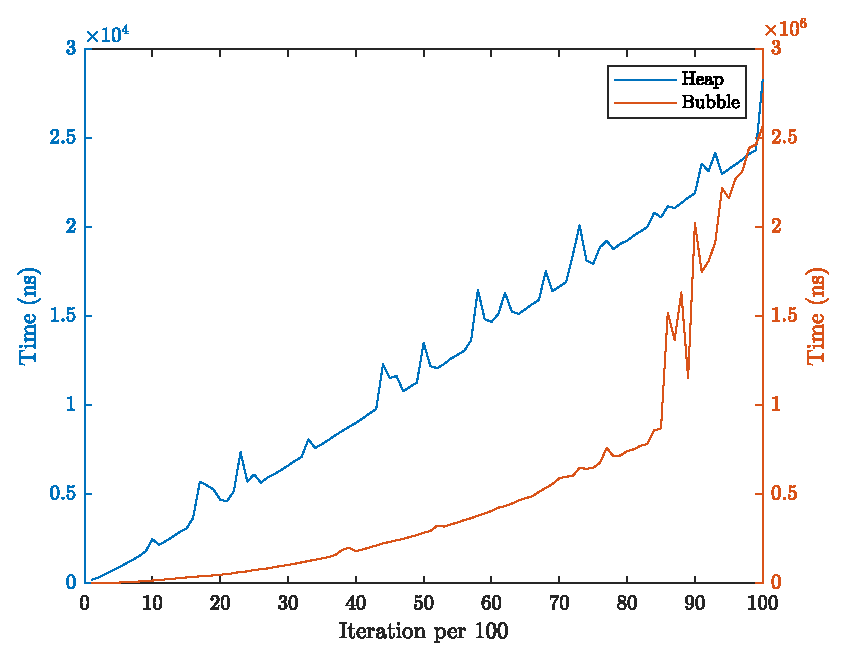
\includegraphics[height=30em]{BubbleHeapSort.eps}
    \caption{Sort timings for heap sort and bubble sort. Note the different time scales.}
\end{figure}

Heap sort has vastly superior sorting times compared to bubble sort. This is because heap sort only operates on the affected sub-trees, giving it time complexity \( O(n*log(n))\). Bubble sort has complexity of \( O(n^2) \). On the first iteration, the largest value is sent to the \( n^{th} \) index. On the second iteration, the second largest value is sent to the \( n - 1 \) index. This process is repeated  \( n  \) times for all contents of the array. This results in a time complexity of \( O(n^2) \). One disadvantage of heap sort is that the data is not perfectly sorted, however with bubble sort the data is perfectly sorted. 

\newpage
\section*{Conclusion}

 \textbf{Part A:}
    Overall, the hash table is more applicable for the database application. The hash table has far superior searching times compared to the doubly linked list. As the number of keys in the database increases, the search performance of the doubly linked list lessens, with complexity \( O(n) \). Compare that to the hash table, where the time complexity for searching stays at \( O(1) \) on average.
    
  \textbf{Part B:}
For the sorting part of this project, heap sort is faster, however it does not perfectly sort all of the data. With time complexity \( O(n * log(n)) \), it vastly out performs bubble sort's complexity of \( O(n ^ 2) \). One advantage of bubble sort is that all of the data is in perfect order. Again, as the number of keys in the database increases, bubble sort's performance drastically reduces compared to heap sort. 

In general, the chosen data structure depends on its operation. A doubly linked list might be more useful than a hash table for a given application, and one sorting algorithm might be chosen over another based on the use case. Knowing which structure to use for a given program is extremely important for efficient algorithms. 

 
\end{document}